\documentclass[tikz, dvisvgm]{standalone}
\usetikzlibrary{patterns}
\usepackage{pgfplots}
\pgfplotsset{compat=1.17}
\usepackage{calc}
% \usepackage{fontspec}
% \setmainfont{Latin Modern}
\usepackage{siunitx}
\sisetup{group-minimum-digits = 3, group-separator = {\,},%
    round-mode = figures, round-precision = 4}
\tikzstyle{altitude}=[align=right,text width=8cm]
\usepackage{fix-cm}
\begin{document}
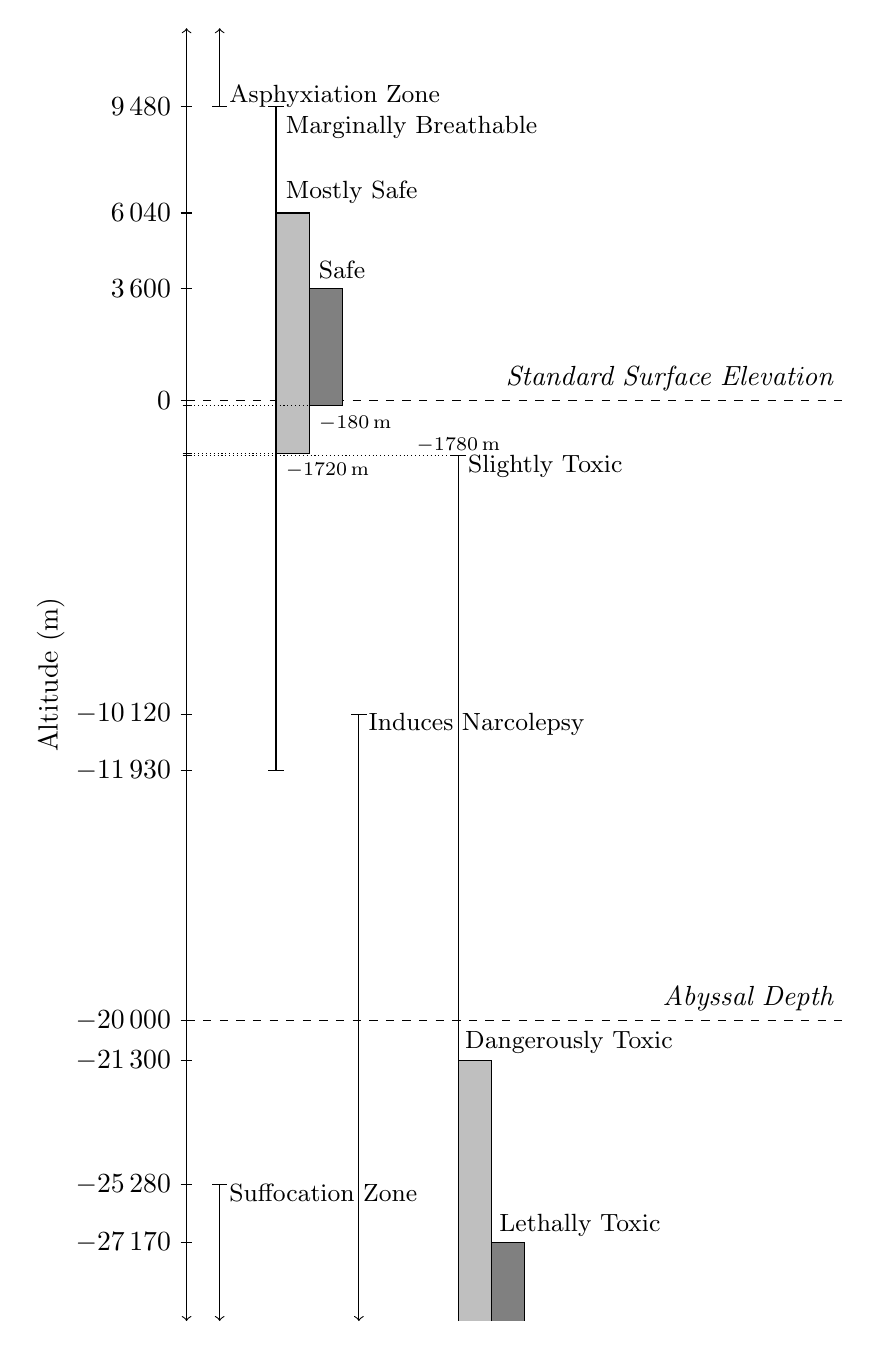
\begin{tikzpicture}%
    \begin{axis}[%
        hide x axis,
        axis y line = left,
        y axis line style = <->,
        ylabel = {Altitude (\si{\m})},
        ylabel style = {yshift=-1.5ex},
        xmin = 0,
        xmax = 20,
        ymin = -29.690,
        ymax = 12,
        xtick=\empty,
        ytick={%
            9.480,%
            6.0401,%
            3.600,%
            0.000,%
            -10.120,%
            -11.930,%
            -20.000,%
            -21.300,%
            -25.280,%
            -27.170%
            },%
        extra y ticks = {-0.180, -1.720, -1.780},
        extra y tick style = {ultra thin, tickwidth=.1cm},
        extra y tick label = \empty,
        yticklabel={%
            \pgfkeys{/pgf/fpu}%
            \pgfmathsetmacro\i{int(\tick * 1000)}%
            \pgfmathprintnumber[fixed relative, precision=4]{\i}%
            \pgfkeys{/pgf/fpu=false}%
        },
        every y tick/.style={color=black, thin},
        width = 10cm,
        height = 18cm,
        /pgf/number format/.cd,
        1000 sep={\,},
    ]

    % plots have +/- .0175 km adjustment to align currectly with the ticks

    % signposts

    % standard surface elevation
    \addplot [color=black, dashed] coordinates {(0,0) (20,0)};
    \node[altitude,above] at (axis cs:10,0) {\it Standard Surface Elevation};

    % abyssal depth
    \addplot [color=black, dashed] coordinates {(0,-20) (20,-20)};
    \node[altitude,above] at (axis cs:10,-20) {\it Abyssal Depth};


    % marginally breathable
    \node[above] (breathUpper) at (axis cs: 2.7, 9.4975) {};
    \node[below] (breathLower) at (axis cs: 2.7, -11.9475) {};
    \draw[|-|] (breathUpper) -- (breathLower);

    \node[below right] at (axis cs: 2.7, 9.480) {\small Marginally Breathable};
    % safe zone
    \addplot [color=black, fill=lightgray] coordinates {%
        (2.7, 6.040) (3.7, 6.040)
        (3.7, -1.72) (2.7, -1.720)
        (2.7, 6.040)
    };
    \node[above right] at (axis cs: 2.7, 6.040) {\small Mostly Safe};
    % optimal zone
    \addplot [color=black, fill=gray] coordinates {%
        (3.7, 3.600) (4.7, 3.600)
        (4.7, -0.180) (3.7, -0.180)
        (3.7, 3.600)
    };
    \node[above right] at (axis cs: 3.7, 3.600) {\small Safe};
    \node[below right] at (axis cs: 3.7, -0.180) {\scriptsize \SI{-180}{\m}};
    \node[below right] at (axis cs: 2.7, -1.720) {\scriptsize \SI{-1720}{\m}};

    % asphyxiation zone
    \node[above] (asphyxUpper) at (axis cs:1, 12) {};
    \node[below] (asphyxLower) at (axis cs:1, 9.4625) {};
    \draw[|->] (asphyxLower) -- (asphyxUpper);
    \node[above right] at (asphyxLower) {\small Asphyxiation Zone};

    % suffocation zone
    \node[above] (suffoUpper) at (axis cs:1, -25.2625) {};
    \node[below] (suffoLower) at (axis cs:1, -29.690) {};
    \draw[|->] (suffoUpper) -- (suffoLower);
    \node [below right] at (suffoUpper) {\small Suffocation Zone};

    % induces narcolepsy
    \node[above] (narcoUpper) at (axis cs: 5.2, -10.1025) {};
    \node[below] (narcoLower) at (axis cs: 5.2, -29.690) {};
    \draw[|->] (narcoUpper) -- (narcoLower);
    \node [below right] at (narcoUpper) {\small Induces Narcolepsy};

    % toxic
    \node[above] (toxicUpper) at (axis cs: 8.2, -1.7625) {};
    \node[below] (toxicLower) at (axis cs: 8.2, -29.690) {};
    \draw[|-] (toxicUpper) -- (toxicLower);
    \node[below right] at (toxicUpper) {\small Slightly Toxic};
    \node at (toxicUpper) {\scriptsize \SI{-1780}{\m}};

    % dangerously toxic
    % \addplot [color=black, mark=-] coordinates {%
    %     (8.2, -21.300)
    %     (8.2, -27.170)
    % };
    % \node[right, mark=-] at (axis cs: 8.2, -21.300) {\small Dangerously Toxic};
    % \node[right] at (axis cs: 8.2, -27.170) {\small Lethally Toxic};

    \addplot [color=black, fill=lightgray] coordinates {%
        (8.2, -29.690)
        (8.2,-21.300) (9.2, -21.300)
        (9.2, -29.690)
    };
    \node[above, xshift=2.8em, yshift=-1pt] at (axis cs: 9.2, -21.300) {\small Dangerously Toxic};

    \addplot [color=black, fill=gray] coordinates {%
        (9.2, -29.690)
        (9.2,-27.170) (10.2, -27.170)
        (10.2, -29.690)
    };
    \node[above, xshift=2em, yshift=-1pt] at (axis cs: 10.2, -27.170) {\small Lethally Toxic};


    % % guides
    % \addplot [color=black, thin, densely dotted] coordinates{(0, 9.480) (2.2, 9.480)};
    % \addplot [color=black, thin, densely dotted] coordinates{(0, 6.040) (3, 6.040)};
    % \addplot [color=black, thin, densely dotted] coordinates{(0, 3.600) (4, 3.600)};
    % \addplot [color=black, thin, densely dotted] coordinates{(0, -10.120) (5.2, -10.120)};
    % \addplot [color=black, thin, densely dotted] coordinates{(0, -11.930) (2.7, -11.930)};
    % \addplot [color=black, thin, densely dotted] coordinates{(0, -21.300) (9.2, -21.300)};
    % \addplot [color=black, thin, densely dotted] coordinates{(0, -25.280) (1, -25.280)};
    % \addplot [color=black, thin, densely dotted] coordinates{(0, -27.170) (10.2, -27.170)};

    % subtick guides
    \addplot [color=black, thin, densely dotted] coordinates{(0, -0.180) (3.7, -0.180)};
    \addplot [color=black, thin, densely dotted] coordinates{(0, -1.720) (2.7, -1.720)};
    \addplot [color=black, thin, densely dotted] coordinates{(0, -1.780) (8.2, -1.780)};
    \end{axis}
\end{tikzpicture}
\end{document}
